\documentclass[11pt,a4paper]{article}
\usepackage[spanish,es-nodecimaldot]{babel}	% Utilizar español
\usepackage[utf8]{inputenc}					% Caracteres UTF-8
\usepackage{graphicx}						% Imagenes
\usepackage[hidelinks]{hyperref}			% Poner enlaces sin marcarlos en rojo
\usepackage{fancyhdr}						% Modificar encabezados y pies de pagina
\usepackage{float}							% Insertar figuras
\usepackage[textwidth=390pt]{geometry}		% Anchura de la pagina
\usepackage[nottoc]{tocbibind}				% Referencias (no incluir num pagina indice en Indice)
\usepackage{enumitem}						% Permitir enumerate con distintos simbolos
\usepackage[T1]{fontenc}					% Usar textsc en sections
\usepackage{amsmath}						% Símbolos matemáticos
\usepackage{listings}
\usepackage{color}

 
\definecolor{codegreen}{rgb}{0,0.6,0}
\definecolor{codegray}{rgb}{0.5,0.5,0.5}
\definecolor{codepurple}{rgb}{0.58,0,0.82}
\definecolor{backcolour}{rgb}{0.99,0.99,0.99}
 
\lstdefinestyle{mystyle}{
    backgroundcolor=\color{backcolour},   
    commentstyle=\color{codegreen},
    keywordstyle=\color{magenta},
    numberstyle=\tiny\color{codegray},
    stringstyle=\color{codepurple},
    basicstyle=\footnotesize,
    breakatwhitespace=false,         
    breaklines=true,                 
    captionpos=b,                    
    keepspaces=true,                 
    numbers=left,                    
    numbersep=5pt,                  
    showspaces=false,                
    showstringspaces=false,
    showtabs=false,                  
    tabsize=2
}
 
\lstset{style=mystyle, language=Python}

% Comando para poner el nombre de la asignatura
\newcommand{\asignatura}{Visión por Computador}
\newcommand{\autor}{José María Sánchez Guerrero}
\newcommand{\titulo}{Cuestionario 2}
\newcommand{\subtitulo}{Clasificación de escenas y objetos}

% Configuracion de encabezados y pies de pagina
\pagestyle{fancy}
\lhead{\autor{}}
\rhead{\asignatura{}}
\lfoot{Grado en Ingeniería Informática}
\cfoot{}
\rfoot{\thepage}
\renewcommand{\headrulewidth}{0.4pt}		% Linea cabeza de pagina
\renewcommand{\footrulewidth}{0.4pt}		% Linea pie de pagina

\begin{document}
\pagenumbering{gobble}

% Pagina de titulo
\begin{titlepage}

\begin{minipage}{\textwidth}

\centering


\includegraphics[scale=0.5]{img/ugr.png}\\

\textsc{\Large \asignatura{}\\[0.2cm]}
\textsc{GRADO EN INGENIERÍA INFORMÁTICA}\\[1cm]

\noindent\rule[-1ex]{\textwidth}{1pt}\\[1.5ex]
\textsc{{\Huge \titulo\\[0.5ex]}}
\textsc{{\Large \subtitulo\\}}
\noindent\rule[-1ex]{\textwidth}{2pt}\\[3.5ex]

\end{minipage}

\vspace{0.5cm}

\begin{minipage}{\textwidth}

\centering

\textbf{Autor}\\ {\autor{}}\\[2.5ex]
\textbf{Rama}\\ {Computación y Sistemas Inteligentes}\\[2.5ex]
\vspace{0.3cm}


\includegraphics[scale=0.3]{img/etsiit.jpeg}

\vspace{0.7cm}
\textsc{Escuela Técnica Superior de Ingenierías Informática y de Telecomunicación}\\
\vspace{1cm}
\textsc{Curso 2019-2020}
\end{minipage}
\end{titlepage}

\pagenumbering{arabic}
\tableofcontents
\thispagestyle{empty}				% No usar estilo en la pagina de indice

\newpage

\setlength{\parskip}{1em}


\section*{Ejercicio 1}
\addcontentsline{toc}{section}{Ejercicio 1}
\textbf{¿Cuál es la transformación más fuerte de la geometría de una escena que puede introducirse al tomar una foto de ella? Dar algún ejemplo.}

Es la \textbf{proyección}, porque es la transformación que menos propiedades de la imagen preserva. Cambia tanto el paralelismo, como las dimensiones,
o los ángulos. Un ejemplo de ello lo podemos ver en el siguiente cubo (todas artistas y ángulos miden lo mismo):
\begin{figure}[H]
\centering
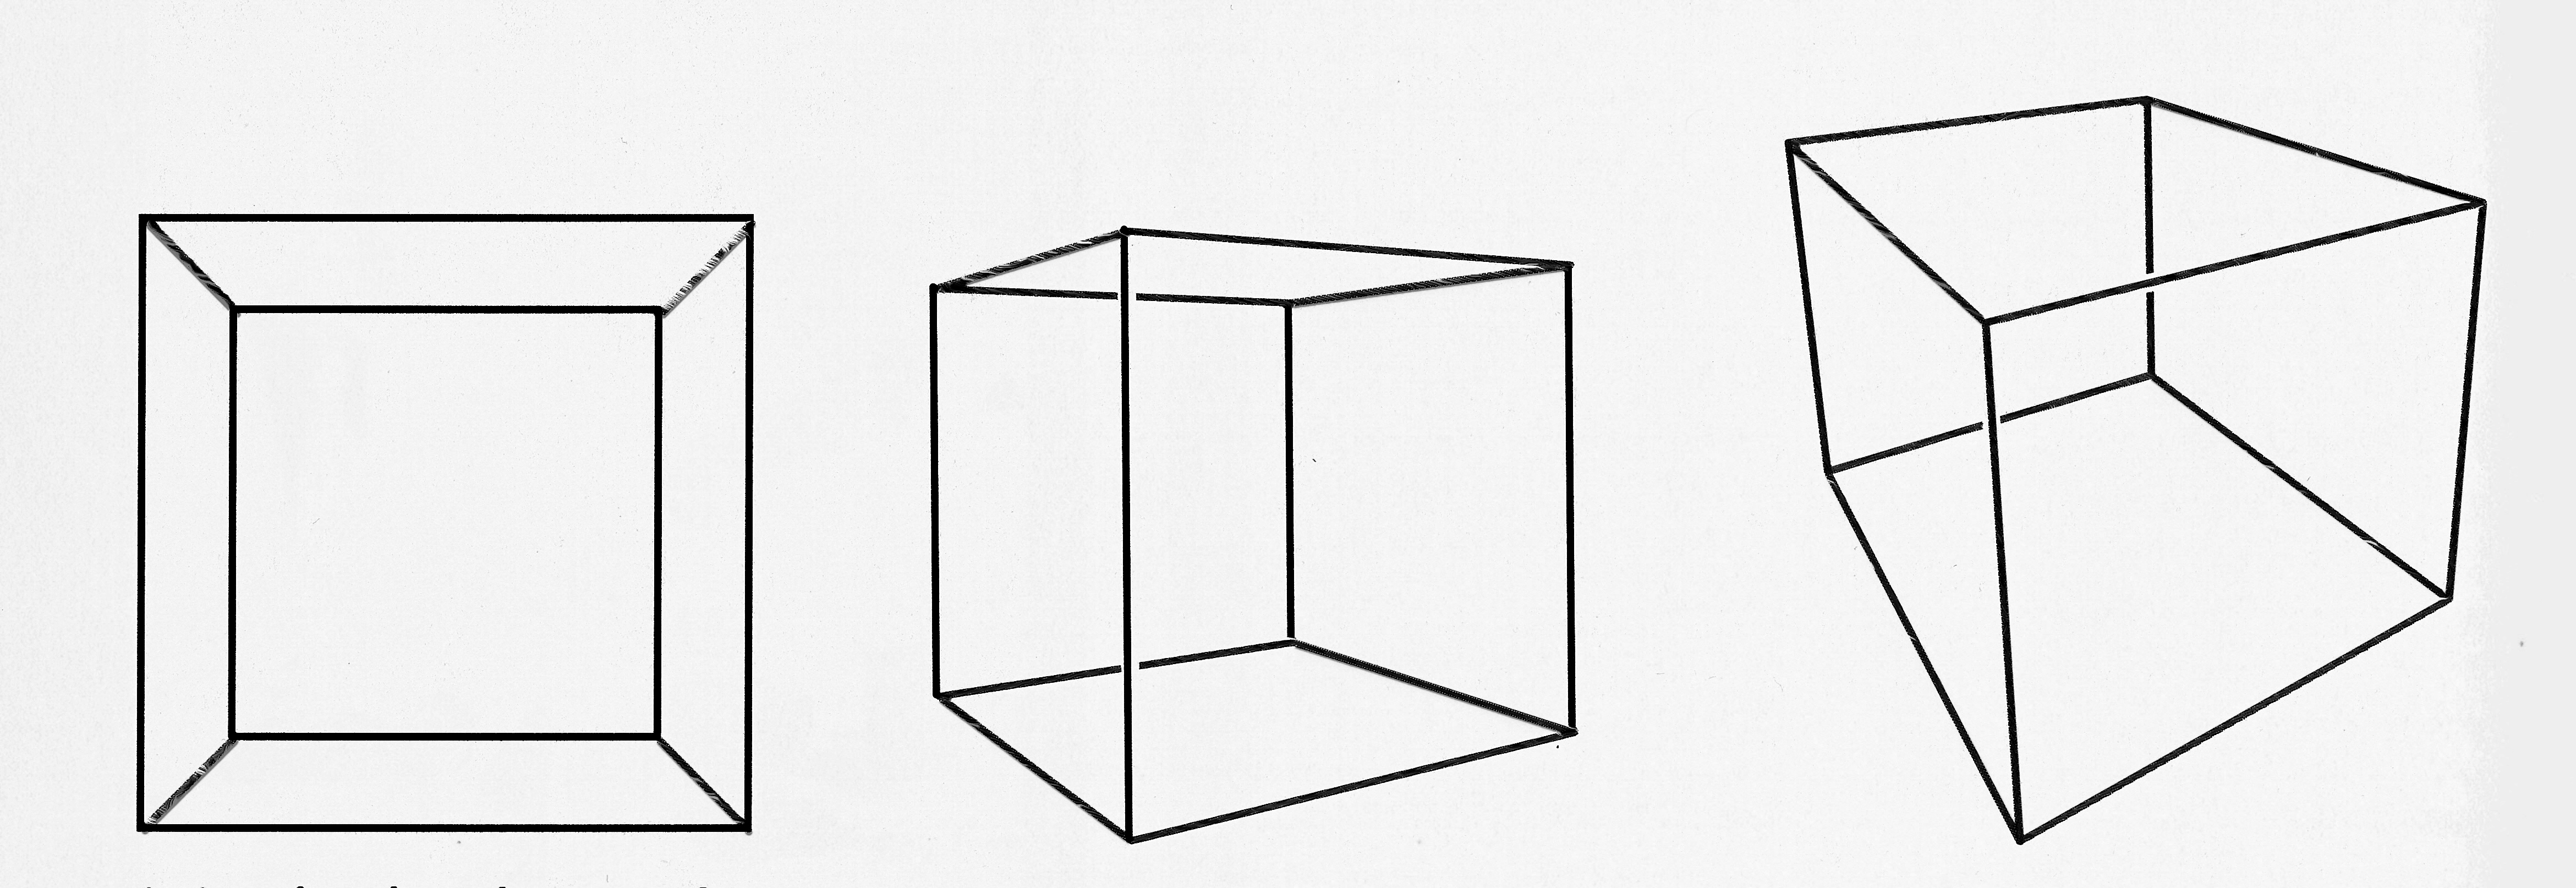
\includegraphics[scale=0.6]{img/cubo.jpg}
\end{figure}

En la imagen de la izquierda podemos ver cómo la cara frontal si conserva los 90º en sus ángulos y si proyectamos sus líneas paralelas al infinito
nunca se cruzarán, pero ya vemos cómo las aristas frontales y posteriores no miden lo mismo, cuando si son iguales. En los demás cubos vemos cómo
ningun ángulo se mantiene con 90º y si proyectamos dos líneas paralelas cualesquiera hasta el infinito, terminarán cruzándose. 



\section*{Ejercicio 2}
\addcontentsline{toc}{section}{Ejercicio 2}
\textbf{¿Por qué es necesario usar el plano proyectivo para estudiar las transformaciones en las imágenes de fotos de escenas? Dar algún ejemplo.}

Porque pese a que no se conserven tamaños o ángulos, si conserva las relaciones de \textbf{incidencia}, es decir, todos los puntos que pertenecen a
una línea, seguirán perteneciendo a esta después de la transformación.

Y de \textbf{cross-ratio}, la cual dice que, dados 4 puntos A, B, C y D pertenecientes a una recta, su \textit{cross-ratio} es igual a $(A,B;C,D)=
(AC\cdot{BD})/(BC\cdot{AD})$. Por ejemplo, si lo llevamos a un plano proyectivo como el siguiente:
\begin{figure}[H]
\centering
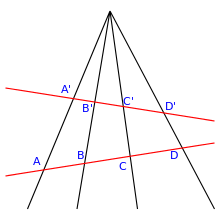
\includegraphics[scale=0.6]{img/plano-proyectivo.jpg}
\end{figure}

Los puntos A, B, C, D y A', B', C', D' están relacionados porque sus relaciones cruzadas, (A, B; C, D) y (A', B'; C', D') son iguales.



\section*{Ejercicio 3}
\addcontentsline{toc}{section}{Ejercicio 3}
\textbf{Sabemos que en el plano proyectivo un punto no existe en el sentido del plano afín, sino que se define por una clase de equivalencia de
vectores definida por $\{k(x,y,1),k\neq{0}\}$. Razone usando las coordenadas proyectivas de los puntos afines de una recta que pase por el (0,0)
del plano afín y verifique que los puntos de la recta del infinito del plano proyectivo son necesariamente vectores del tipo (*,*,0) con *=cualquier
número.}

Si tenemos en cuenta que *=cualquier número, por ejemplo $a$, cualquier punto representado en el plano proyectivo vendría dado por:
\begin{equation*}
(ax, ay, 1) = (x,y,\frac{1}{a})
\end{equation*}
Un punto en el infinito del plano proyectivo hace que $a=\infty$ y en consecuencia que $\frac{1}{a} = 0$, y por tanto podemos decir que su vector de
coordenadas es del tipo $(x,y,0)$.



\section*{Ejercicio 4}
\addcontentsline{toc}{section}{Ejercicio 4}
\textbf{¿Qué propiedades de la geometría de un plano quedan invariantes cuando se toma una foto de él? Justificar la respuesta.}

Dependiendo de la foto que hayamos tomado, las propiedades que quedan invariantes serán unas u otras. Si tomamos la siguiente imagen de las
transparencias como guía, las transformaciones que no se producen son la de su misma fila más las que aparecen debajo:
\begin{figure}[H]
\centering
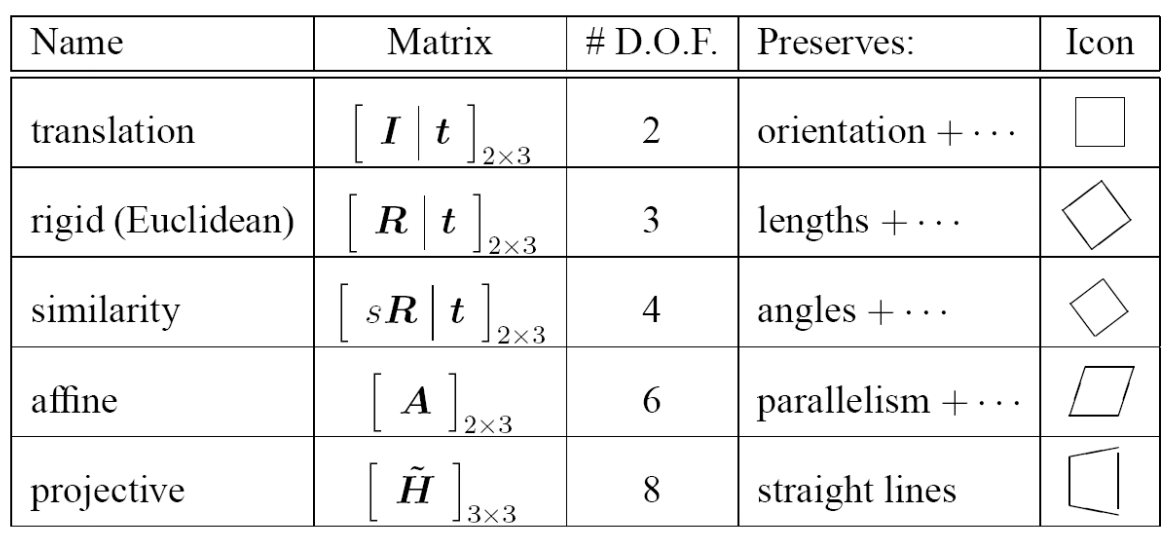
\includegraphics[scale=0.4]{img/transformaciones.png}
\end{figure}

Por ejemplo, teniendo en cuenta las fotografía de abajo, si tomamos la de la izquierda, vemos cómo la foto no ha sufrido cambios y las propiedades
que se conservan son la orientación + tamaños + ... + líneas rectas. Mientras que si tomamos la imagen de la derecha, que es una foto en el plano
proyectivo, sólo conserva las propiedades de éste (como pueden ser la incidencia o el \textit{cross-ratio} comentados en el ejercicio 2).
\begin{figure}[H]
\centering
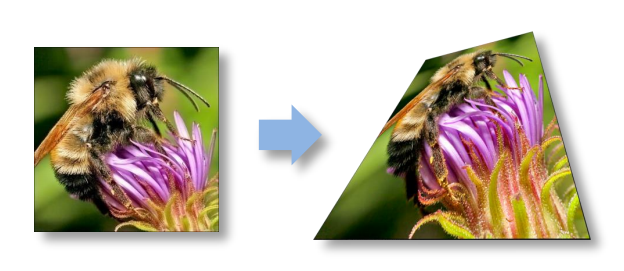
\includegraphics[scale=0.6]{img/transformaciones2.png}
\end{figure}



\section*{Ejercicio 5}
\addcontentsline{toc}{section}{Ejercicio 5}
\textbf{En coordenadas homogéneas los puntos y rectas del plano se representan por vectores de tres coordenadas (notados x y l respectivamente), de
manera que si una recta contiene a un punto se verifica la ecuación $x^Tl=0$, es decir $(x_1,x_2,x_3)\begin{pmatrix}a\\b\\c\end{pmatrix} = 0$.
Considere una homografía H que transforma vectores de puntos, $x' = Hx$. Dado que una homografía transforma vectores de tres coordenadas también
existen homografías G para transformar vectores de rectas $l' = Gl$. Suponga una recta $l$ y un punto $x$ que verifican $x^Tl=0$ en el plano proyectivo
y suponga que conoce una homografía H que transforma vectores de puntos. En estas condiciones ¿cuál es la homografía G que transforma los vectores de
las rectas? Deducirla matemáticamente.}

Para calcular una homografía G tal que $l'=Gl$, tendremos en cuenta que para todos los puntos de la recta $l$, si aplicamos una homografía conocida H
($x'=Hx$) obtenemos una nueva recta $l'$. Si cada punto $x'$ debe de estar contenido en la recta $l'$, podemos verificar que $(x')^Tl'=0$.

Si ahora consideramos las transformaciones que realizan las homografías H y G en los vectores de puntos y rectas, respectivamente, tenemos que:
\begin{equation*}
(x')^Tl' = (Hx)^T Gl = x^T H^T Gl = 0
\end{equation*}

Por otra parte, si hacemos que $H^TG=I$, siendo I la matriz identidad, podremos llegar a donde queríamos:
\begin{equation*}
x^T H^T Gl = x^T (H^T G) l = x^T (I) l = x^T l = 0
\end{equation*}

Por último, ya sólo nos queda despejar la G de forma que:
\begin{equation*}
H^T G = I \rightarrow G = (H^-1)^T
\end{equation*}

\section*{Ejercicio 6}
\addcontentsline{toc}{section}{Ejercicio 6}
\textbf{¿Cuál es el mínimo número de escalares necesarios para fijar una homografía general? ¿Y si la homografía es afín? Justificar la respuesta}


\section*{Ejercicio 7}
\addcontentsline{toc}{section}{Ejercicio 7}
\textbf{Defina una homografía entre planos proyectivos que haga que el punto (3,0,2) del plano proyectivo-1 se transforme en un punto de la recta del
infinito del plano proyectivo-2? Justificar la respuesta.}


\section*{Ejercicio 8}
\addcontentsline{toc}{section}{Ejercicio 8}
\textbf{}

\section*{Ejercicio 9}
\addcontentsline{toc}{section}{Ejercicio 9}
\textbf{¿Cuáles son las propiedades necesarias y suficientes para que una matriz defina un movimiento geométrico no degenerado entre planos? Justificar
la respuesta}


\section*{Ejercicio 10}
\addcontentsline{toc}{section}{Ejercicio 10}
\textbf{¿Qué información de la imagen usa el detector de Harris para seleccionar puntos? ¿El detector de Harris detecta patrones geométricos o fotométricos?
Justificar la contestación.}


\section*{Ejercicio 11}
\addcontentsline{toc}{section}{Ejercicio 11}
\textbf{¿Sería adecuado usar como descriptor de un punto Harris los valores de los píxeles de su región de soporte? Identifique ventajas, inconvenientes y
mecanismos de superación de estos últimos.}


\section*{Ejercicio 12}
\addcontentsline{toc}{section}{Ejercicio 12}
\textbf{Describa un par de criterios que sirvan para seleccionar parejas de puntos en correspondencias (“matching”) a partir de descriptores de regiones
extraídos de dos imágenes. ¿Por qué no es posible garantizar que todas las parejas son correctas?}


\section*{Ejercicio 13}
\addcontentsline{toc}{section}{Ejercicio 13}
\textbf{Cual es el objetivo principal del uso de la técnica RANSAC en el cálculo de una homografía. Justificar la respuesta}


\section*{Ejercicio 14}
\addcontentsline{toc}{section}{Ejercicio 14}
\textbf{Si tengo 4 imágenes de una escena de manera que se solapan la 1-2, 2-3 y 3-4. ¿Cuál es el número mínimo de parejas de puntos en correspondencias
necesarios para montar un mosaico? Justificar la respuesta}


\section*{Ejercicio 15}
\addcontentsline{toc}{section}{Ejercicio 15}
\textbf{¿En la confección de un mosaico con proyección rectangular es esperable que aparezcan deformaciones geométricas de la escena real? ¿Cuáles y por qué?
¿Bajo qué condiciones esas deformaciones podrían no estar presentes? Justificar la respuesta.}

\end{document}